% !TEX TS-program = pdflatex
% !TEX encoding = UTF-8 Unicode

% This is a simple template for a LaTeX document using the "article" class.
% See "book", "report", "letter" for other types of document.

\documentclass[11pt]{article} % use larger type; default would be 10pt

\usepackage[utf8]{inputenc} % set input encoding (not needed with XeLaTeX)
\usepackage{wrapfig}
%%% Examples of Article customizations
% These packages are optional, depending on whether you want the features they provide.
% See the LaTeX Companion or other references for full information.

%%% PAGE DIMENSIONS
\usepackage{geometry} % to change the page dimensions
\geometry{a4paper} % or letterpaper (US) or a5paper or....
% \geometry{margin=2in} % for example, change the margins to 2 inches all round
% \geometry{landscape} % set up the page for landscape
% read geometry.pdf for detailed page layout information

\usepackage{graphicx} % support the \includegraphics command and options
\usepackage{url} % better links representation, o così dicono

% \usepackage[parfill]{parskip} % Activate to begin paragraphs with an empty line rather than an indent

%%% PACKAGES
\usepackage{amsmath}
\usepackage{booktabs} % for much better looking tables
\usepackage{array} % for better arrays (eg matrices) in maths
\usepackage{paralist} % very flexible & customisable lists (eg. enumerate/itemize, etc.)
\usepackage{verbatim} % adds environment for commenting out blocks of text & for better verbatim
\usepackage{subfig} % make it possible to include more than one captioned figure/table in a single float
% These packages are all incorporated in the memoir class to one degree or another...
\usepackage{listings,multicol}
\usepackage{caption}

\usepackage{graphicx}
\graphicspath{ {./images/} }

\usepackage{mathpartir}

%%% HEADERS & FOOTERS
\usepackage{fancyhdr} % This should be set AFTER setting up the page geometry
\pagestyle{fancy} % options: empty , plain , fancy
\renewcommand{\headrulewidth}{0pt} % customise the layout...
\lhead{}\chead{}\rhead{}
\lfoot{}\cfoot{\thepage}\rfoot{}

%%% SECTION TITLE APPEARANCE
\usepackage{sectsty}
\allsectionsfont{\sffamily\mdseries\upshape} % (See the fntguide.pdf for font help)
% (This matches ConTeXt defaults)

\usepackage[usenames,dvipsnames]{xcolor}
\usepackage{hyperref} % To refer a link (website)
\hypersetup{%
  colorlinks=true,% hyperlinks will be coloured
  %linkcolor={BrickRed},% hyperlink text will be green
  linkbordercolor=BrickRed,
  citebordercolor=White,
  urlbordercolor=White,
  runbordercolor=White,
  menubordercolor=White,
  filebordercolor=White,
 % urlcolor={BrickRed},
%filecolor={White},
%citecolor={BrickRed},
allcolors={BrickRed}
%allbordercolors={BrickRed}
}

\makeatletter
\Hy@AtBeginDocument{%
  \def\@pdfborder{0 0 1}% Overrides border definition set with colorlinks=true
  \def\@pdfborderstyle{/S/U/W .5}% Overrides border style set with colorlinks=true
                                % Hyperlink border style will be underline of width 1pt
}
\makeatother

%%% ToC (table of contents) APPEARANCE
\usepackage[nottoc,notlof,notlot]{tocbibind} % Put the bibliography in the ToC
\usepackage[titles,subfigure]{tocloft} % Alter the style of the Table of Contents

\renewcommand{\cftsecfont}{\rmfamily\mdseries\upshape}
\renewcommand{\cftsecpagefont}{\rmfamily\mdseries\upshape} % No bold!

\setlength\parindent{0pt} % Set noindent for the whole document
\newcommand{\ES}{\textcolor{red}}


\usepackage{tikz}
\usetikzlibrary{shapes,trees,fit,decorations.pathreplacing,arrows.meta}

\definecolor{codegreen}{rgb}{0,0.6,0}
\definecolor{codegray}{rgb}{0.5,0.5,0.5}
\definecolor{codepurple}{rgb}{0.58,0,0.82}
\definecolor{backcolour}{rgb}{0.95,0.95,0.92}

\lstdefinestyle{mystyle}{
    backgroundcolor=\color{backcolour},   
    commentstyle=\color{codegreen},
    keywordstyle=\color{magenta},
    numberstyle=\tiny\color{codegray},
    stringstyle=\color{codepurple},
    basicstyle=\ttfamily\footnotesize,
    breakatwhitespace=false,         
    breaklines=true,                 
    captionpos=b,                    
    keepspaces=true,                 
    numbers=left,                    
    numbersep=5pt,                  
    showspaces=false,                
    showstringspaces=false,
    showtabs=false,                  
    tabsize=2
}

\lstset{style=mystyle}
%%% END Article customizations

\begin{document}
%\maketitle

%%% Title page
\begin{titlepage}
	\topskip0pt
	%\vspace*{\fill}
	\centering
	
\includegraphics[width=\textwidth]{logo.png}\\
	\vspace*{1cm}
	\Large \textsc{Second Cycle Degree in Computer Science}
	
	\vspace*{10mm}
	\hrule width \hsize \kern 1mm \hrule width \hsize height 2pt
	\vspace*{5mm}
	\Huge \emph{\textbf{Asset Language}}\\
	\large \emph{\textbf{Compilers and Interpreters  Course Project}}\\
	\large \emph{\textbf{Report on design choices}}
	\vspace*{5mm}
	\hrule width \hsize height 2pt
	\vspace*{1mm}
	\hrule width \hsize \kern 1mm
	
	\vspace*{10mm}
	\begin{minipage}{0.45\textwidth}
		\begin{flushleft} \Large
			\emph{Students:}\\
			\Large \textbf{Giuseppe \textsc{CAPUTO}}\\
			\Large \textbf{Alberto \textsc{PAPARELLA}}
			\Large \textbf{Gabriele \textsc{SPINA}}
		\end{flushleft}
	\end{minipage}	
	\begin{minipage}{0.45\textwidth}
		\begin{flushright} \Large
			\emph{Professor:}\\
			\Large \textbf{Prof. Cosimo \textsc{LANEVE}}
		\end{flushright}
	\end{minipage}
	
	\vspace*{15mm}
	\Large \textsc{Academic Year $2021-2022$}
\end{titlepage}

% Table of contents
\addtocontents{toc}{~\hfill\textbf{Page}\par}	% https://texblog.org/2011/09/09/10-ways-to-customize-tocloflot/
\clearpage
\tableofcontents
\thispagestyle{empty}
\addtocontents{toc}{\protect\thispagestyle{empty}}	% http://tex.stackexchange.com/questions/2995/removing-page-number-from-toc
\newpage

\section{Introduction}
This report will discuss the implementation choices related to the design of a compiler and relative interpreter for a specific programming language, called \emph{AssetLan} (i.e., Asset Language). 

\medskip

\emph{Asset Language} is a simple imperative language with assets, where parameters could be either {\emph standard} or {\emph assets}, with recursion and without mutual recursion. Regarding the semantics, two types of operations are allowed on a parameter defined as an {\emph asset}, and it is legit to use them only in a function. To this aim, a function can be declared  with {\emph assets} in the following way:
\begin{verbatim}
    void f(int a, bool b)[asset u, asset v] { body }
\end{verbatim} 
and called as: 
\begin{verbatim}
    f(5,true)[x,y]
\end{verbatim}
At the time of the call, assets \verb|x| and \verb|y| are emptied and their values are assigned respectively to the formal parameters \verb|u| and \verb|v|; therefore, after the call, the values of assets \verb|x| and \verb|y| are both equal to 0.

\medskip

The value of an \emph{asset} can \textbf{only} be moved using the two aforementioned operations, more specifically: 
\begin{itemize}
\item \textbf{Move operation} (\verb|x -o z|): the value of the parameter \verb|x| is added to the value of the parameter \verb|z| and stored in \verb|z|, then the value of the parameter \verb|x| is set to 0;
\item \textbf{Transfer operation} (\verb|transfer x|): this operation transfers the value of the asset \verb|x| to the caller of the function, then its value is set to 0.
\end{itemize}

\section{Usage}

\subsection{Launching from command line}

Tu use the compiler, go to folder \verb|/src| and compile all java files in the sub directories with \verb|javac */*.java| (it is assumed that antlr4 has already been added to java classpath).
To execute the compiler on a file with \verb|.al| extension, place the file in the \verb|/src| directory and call the Test class, which contains the main function, as follows: \verb|java mainpackage.Test input.al|, where \verb|input.al| is an example of file name.

\subsection{Launching from IDE}
To launch the analysis from an IDE (e.g., Eclipse), open the \verb|src| folder as a new project and add antlr4 to the build path according to the IDE settings. Then, create a new launch configuration to tell the IDE where the main class is, which can be found int \verb|/src/mainpackage/Test.java|, and the command line arguments, in this case the input file with \verb|.al| extension (e.g., \verb|input.al|).

\section{Exercises}
\label{sec:exercices}
The following exercises were used as guidelines/objectives for the design of the compiler:

\begin{enumerate}
\item \textbf{Lexical Errors}: the lexical analyzer must return the list of lexical errors in an output file. 
\item \textbf{Symbol Table}: implement the table of symbols as a list of hash-tables or a hash-table of lists, in order to check errors related to:
\begin{itemize}
\item undeclared functions/variables;
\item multiple declarations of functions/variables in the same environment.
\end{itemize}
\item \textbf{Type checking}: implement a semantic analysis that verify:
\begin{itemize}
\item the type correctness;
\item the liquidity of the program:
\begin{itemize}
\item for each function, the asset formal parameters must be $0$ at the end of his execution;
\item at the end of the program all asset fields are $0$.
\end{itemize} 
\end{itemize}
\item \textbf{Code Generation and Interpreter}: define a bytecode language to execute programs in AssetLan and implement the interpreter. In particular:
\begin{itemize}
\item the bytecode must have instructions for a stack machine that memorize in ad-hoc register(\$a0) the value of the last instruction calculated;
\item implement the interpreter for that bytecode;
\item compile and execute the programs of the high level language.
\end{itemize} 
\end{enumerate}

\subsection{Lexical Errors}
In order to redirect the errors of the lexer to an output (log) file, one should override the base error handling strategy of ANTLR, which, by default, redirects the errors to the standard error (i.e., the console). To change the destination and, eventually, the content of error messages, one should provide an implementation of an \textsc{ANTLRErrorListener} subclass; Figure~\ref{fig:err} shows the structure of the classes involved in the error handling phase.
\begin{figure}
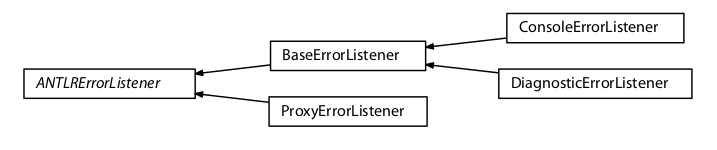
\includegraphics[width=0.95\textwidth]{errorListener.png}
\caption{Internal structure for error handling\cite{reference}.}
\label{fig:err}
\end{figure}   
More specifically, \textsc{ANTLRErrorListener} provides a \textsc{syntaxError()} method that applies to both the lexer and the parser, which receives all sorts of information about the location of the error, as well as the error message and which recognizer caught the error (i.e., if the error occurred during the lexical or the syntactic analysis).   

\medskip

The proposed solution consists of a class, called \textsc{TestLexerListner}, which extends the \textsc{BaseErrorListener} class in order to override the \textsc{syntaxError()} method and redirect his output to a log file, named \verb|log.txt|. Furthermore, for each error, it prints the date and time at which it occurred, so that it is possible to distinguish between errors coming from different compilation executions. 

\medskip

At this point, one can simply remove the \textsc{ConsoleErrorListener} (i.e., the default strategy) for the lexer and bind the custom listener instead, adding the following lines to the main function intended to launch the analysis and relative compilation (in the project, defined in the \verb|Test| class, implemented in \verb|src/mainpackage/Test.java|):
\begin{lstlisting}
    lexer.removeErrorListeners();
    lexer.addErrorListener(new TestLexerListener());
\end{lstlisting}

\medskip

A lexical error is defined as a sequence of characters that does not match the pattern of any token. In our language, this can only happen when the lexer founds a character which is not defined in the grammar, and therefore it cannot derive the relative token. 

\medskip

The following examples show the output messages printed to the \verb|log.txt| file when a lexical error is found:
\begin{enumerate}
\item
	\begin{itemize}
		\item Code tested: \begin{lstlisting}
int a = "s";   
f()[]		\end{lstlisting}
		\item Output on \textsc{log.txt}: \begin{lstlisting}
20-04-2022 15:33:13: 
    Found Lexical error at line 1 at position 8: 
    token recognition error at: '"'
20-04-2022 15:33:14: 
    Found Lexical error at line 1 at position 10: 
    token recognition error at: '"'		\end{lstlisting}
	\end{itemize}
\item
\begin{itemize}
\item Code tested: \begin{lstlisting}
int main()[]{}
ma$n()[]
\end{lstlisting}
\item Output on \textsc{log.txt}: \begin{lstlisting}
20-04-2022 15:48:56: 
    Found Lexical error at line 2 at position 2: 
    token recognition error at: '$'
\end{lstlisting}
\end{itemize}
\item
	\begin{itemize}
	\item Code tested: \begin{lstlisting}
int a:
f()[]	\end{lstlisting}
	\item Output on \textsc{log.txt}: \begin{lstlisting}
20-04-2022 15:55:52: 
    Found Lexical error at line 1 at position 5: 
    token recognition error at: ':'	\end{lstlisting}
	\end{itemize}
\end{enumerate}

\clearpage

\subsection{Symbol Table}
The choice of the data structure for the symbol table fell on the list of hash-tables because an excessive level of nesting in the code is not expected. This is due to the fact that the grammar of the language does not allow the definition of {code blocks}~\cite{codeblocks} (i.e., using curly brackets to define a new scope explicitly, as in SimpLanPlus) and mutual recursion is not conceived; therefore, the only way to enter in a new scope is the definition of a new function. That leads to a language that frequently enters and exits scopes, so it has been decided to opt for a solution that could reduce the complexity of these particular operations, accepting a higher complexity for the look-up of an identifier. Given the implementation of a symbol table as a list of hash-tables, the cost for entering and exiting a scope is \(O(1)\), while the cost for the look-up operation is \(O(depth_{nesting})\).

\medskip

The symbol table has been declared as a private field in a specific class, called \textsc{Environment}. In order to access/modify it, the following methods have been implemented:
\begin{itemize}
\item \textsc{enterScope()}: increases the nesting level and adds a new entry (i.e., an hash-table) to the list. 
\item \textsc{exitScope()}: decreases the nesting level and removes the last hash-table from the list.
\item \textsc{getScope(nestingLevel)}/\textsc{getCurrentScope()}: returns the scope relative to the specified nesting level/relative to the current nesting level.
\item \textsc{addEntry(type, identifier)}: adds an entry with specified type and id to the hash-table relative to the current scope.
\item \textsc{getNestingLevel()}: getter for nesting level field.
\item \textsc{checkDeclaration(identifier, nestingLevel)}: checks if the symbol has been declared in the specified scope (retrieved from nesting level). 
\item \textsc{lookup(identifier)}: look-up for the declaration of a given id in the current scope or an enclosing one. 
\end{itemize}

\medskip

To manage the symbol table, it is necessary to visit the Abstract Syntax Tree in order to insert the declarations of variables / functions / assets within the data structure. To this aim, the \textsc{AssetLanBaseVisitor} class has been extended to override the auto-generated methods meant to visit the AST. For each rule in the grammar, it has been defined a new class representing the relative node of the tree with its specific components and methods. Among these, \textsc{checkSemantics(environment)} searches for semantic errors, such as multiple declarations of variables and functions, as well as undeclared ones.

\medskip

In the \textsc{AssetLanBaseVisitor} there is a visit method for each rule in the grammar meant to construct the relative node with the help of the ANTLR's rule contexts. 

\medskip

The following example shows the output for a program which contains both types of errors (one multiple declaration error and one usage of undeclared variable error):

\begin{enumerate}
\item
	\begin{itemize}
		\item Code tested: \begin{lstlisting}
int a;
asset b;
int main(int a)[asset c]{
    int a;
    c -o d;
}
main()[2]
		\end{lstlisting}
		\item Output on console: \begin{lstlisting}
You had: 2 errors:
	Error when declaring variable of id a,
	Id already used for declaration in the same scope
	
	Asset d has not been declared
		\end{lstlisting}
		
	The first error is caused by the declaration of variable \verb|a| at line 4, which has already been declared as parameter in the function.
	The second error is caused by the fact that asset \verb|d| has never been declared.
	\end{itemize}
\end{enumerate}

\subsection{Type Checking}
To implement type management, the semantic rules for managing and verifying the environment are shown below. After the implementation of the conditions imposed by the inference rules on the individual nodes, a test phase has been executed.

\subsubsection{Inference Rules}
Each entry of the symbol table ($ \Gamma $) will be of one of those forms:

\begin{equation}
\Gamma, n :
	\begin{cases}
	Id \rightarrow ( T \lor A, n' ) \qquad & \text{if the } Id \text{ refers to a variable} \\ \\
	\begin{split}
	Id & \rightarrow  (x_1 \rightarrow T_1,\cdots
          							 x_n \rightarrow T_n) \rightarrow \\
          		   &		\rightarrow (y_1 \rightarrow A_1,\cdots
          							 y_m \rightarrow A_M) \rightarrow \\
          		   &		\rightarrow T 
	\end{split} \qquad & \text{if the } Id \text{ refers to a function}
	\end{cases}
\end{equation}
\captionof*{figure}{Where $T=\{int, bool\}$, $A=\{asset\}$, and $n, n'$ represents the offsets.}

To handle the effects of the liquidity, it has been used the $\Sigma$ environment that is composed as follows: \\ 
\[
\Sigma : Id \rightarrow \mathcal{B} \qquad
\text{ where, } \mathcal{B} =\{ \bot, f , \top \}
\]
The analysis of the effects is performed only on assets, when it is empty is $\bot$, when filled up is $f$(full), and when is undefinable is $\top$. That is, at the end of a program you can check if all the assets variables are $\bot$; so the program can be defined as liquid.

\medskip

\begin{equation}
\begin{split}
& \Gamma, n \models F  : \Gamma', n' \quad \text{Field} \qquad \qquad \quad 
\Gamma, n \models Fn : \Gamma', n' \quad \text{Function} \\
& \Gamma, n \models D : \Gamma', n' \quad \text{Declaration} \qquad 
\Gamma, n \models Ad : \Gamma', n' \quad \text{Asset declaration} \\
& \Gamma \models St : T \lor A \quad \text{Statement} \qquad \qquad
\Gamma \models A : T \quad \quad \text{Assignment} \\
& \Gamma \models M : A \quad \text{Move} \qquad \qquad \qquad \quad
\Gamma \models P   \quad \text{Print} \\
& \Gamma \models Tr : A \quad \text{Transfer} \qquad \qquad \qquad
\Gamma, n \models R : T  \quad \text{Return} \\
& \Gamma \models Ite : T \quad \text{If then else} \qquad \qquad 
\Gamma \models Call : T \quad \text{Function call} \\
& \Gamma \models InitC : T \quad \text{Init call} \qquad \qquad 
\Gamma \models Exp : T \lor A \quad \text{Expression} \\
\end{split}
\end{equation}
\captionof*{figure}{There are the base rules}

\medskip 

\[
\inferrule*[right=(Prg)]
{[\,],0 \models F : \: \Gamma, n \\ \Gamma,n \models Ad : \: \Gamma_1,n_1 \\ \Gamma_1, n_1 \models Fn : \: \Gamma_2, n_2 \\ \Gamma_2, n_2 \models InitC : \:T }
{[\,], 0 \models F* Ad* Fn* InitC : \: T} 
\]
\captionof*{figure}{Program rule, start from empty environment}

\medskip

\[
\inferrule*[right=(IntF)]
{Id \notin Dom(\Gamma) \\ \Gamma \models E : \: int}
{\Gamma, n \models int \: Id = E; : \: \Gamma[Id\rightarrow(int, n)], n+4}
\inferrule*[right=(BoolF)]
{Id \notin Dom(\Gamma) \\ \Gamma \models E : \: bool}
{\Gamma, n \models bool \: Id = E; : \: \Gamma[Id\rightarrow(bool, n)], n+1}
\]
\captionof*{figure}{Rules for Field}

\medskip

\[
\inferrule*[right=(Asset)]
{Id \notin Dom(\Gamma) }
{\Gamma, n \models asset \: Id ; : \: \Gamma[Id\rightarrow(A, n)], n+4}
\]
\captionof*{figure}{Asset rule}

\medskip

\[
\inferrule*[right=(Fun)]{
Id \notin Dom(\Gamma) \\ 
\Gamma \bullet [\,],0 \models D : \: \Gamma \bullet \Gamma',n' \\ 
\Gamma',n' \models A : \: \Gamma'',n'' \:
\cdots}
{\Gamma,n \models T \: Id (D ) [A ] \{D_1  \: S \}:  \: \cdots}
\]

\[
\inferrule*[right=(Fun)]{\cdots \: \Gamma'',n'' \models D_1 : \: \Gamma''',n'''\\
\inferrule*[right=(S-Stm)]{
	\inferrule*[rightstyle={\tiny \sc}, right=(A statement must be return), leftskip=2em,rightskip=2em, vdots=1.5em]{\Gamma''',n''' \models E : \: T}		     {\Gamma''',n''' \models return \: E: \: T}
	}
	{\Gamma''',n''' \models S }
}
{\cdots \: \Gamma[Id\rightarrow(x_1\rightarrow T_1 \cdots x_n\rightarrow T_n)\rightarrow(y_1\rightarrow A_1 \cdots y_n\rightarrow A_n)\rightarrow T], n}
\]
\captionof*{figure}{Rule for Function Declaration}

\medskip

\[
\inferrule*[right=(Dec-i)]
{Id \notin Dom(\top(\Gamma)) \\ \Gamma \models E : \: int}
{\Gamma, n \models int \: Id = E; : \: \Gamma[Id\rightarrow(int, n)], n+4}
\inferrule*[right=(D-Dec)]
{\Gamma,n \models D : \Gamma'',n'' \\
 \Gamma'',n'' \models D': \: \Gamma',n'}
{\Gamma,n \models D D' : \: \Gamma',n'}
\]
\captionof*{figure}{Rule for multiple declarations (Dec in the grammar, rule for bool is immediate to retrieve)}

\medskip

\[
\inferrule*[right=(A)]
{Id \notin Dom(\top(\Gamma)) }
{\Gamma, n \models asset \: Id ; : \: \Gamma[Id\rightarrow(A, n)], n+4}
\inferrule*[right=(A-Dec)]
{\Gamma,n \models A : \Gamma'',n'' \\
 \Gamma'',n'' \models A': \: \Gamma',n'}
{\Gamma,n \models A A' : \: \Gamma',n'}
\]
\captionof*{figure}{Rule for multiple assets declarations (ADec in the grammar)}

\medskip

\[
\inferrule*[right=(Stm)]
{ass \\ mv \\ pr \\ tr \\ ret \\ ite \\ call}
{\Gamma,n \models St: \: T}
\]
\[
\inferrule*[right=(S-Stm)]
{\Gamma,n \models S : \: T \\ \Gamma,n \models S' : \: T_1\\ }
{\Gamma,n \models S S' :\:T_1}
\]
\captionof*{figure}{Rule for statement, multiple statements}

\[
\inferrule*[right=(Asm)]
{Id \in Dom(\Gamma) \\ \Gamma(Id)=T \\ \Gamma \models E : \: T}
{\Gamma \models Id = E : \: T}
\]
\[
\inferrule*[right=(A-Asm)]
{Id \in Dom(\Gamma) \\ \Gamma(Id)=int \\ \Gamma \models E : \: A}
{\Gamma \models Id = E : \: int}
\]
\captionof*{figure}{Assignment rules, it is legit to assign the value in an asset to an integer}

\[
\inferrule*[right=(Mv)]
{Id_1 \in Dom(\Gamma) \\ \Gamma(Id_1)=A \\ Id_2 \in Dom(\Gamma) \\ \Gamma(Id_2)=A}
{\Gamma \models Id_1 -o \: Id_2 }
\]
\captionof*{figure}{Move operation rule}

\medskip

\[
\inferrule*[right=(Pr)]
{\Gamma \models E : T \lor A}
{\Gamma \models print E }
\]
\captionof*{figure}{Print rule}

\medskip

\[
\inferrule*[right=(Tr)]
{Id \in Dom(\Gamma) \\ \Gamma(Id) = A}
{\Gamma \models transfer \: Id }
\]
\captionof*{figure}{Transfer rule}

\medskip

\[
\inferrule*[right=(Ret)]
{\Gamma \models E : \: T}
{\Gamma \models return \: E : \: T}
\inferrule*[right=(Ret-A)]
{\Gamma \models E : \: A}
{\Gamma \models return \: E : \: int}
\]
\captionof*{figure}{Return rule, it is possible to return the value in an asset, so the return type will be int (!! When this happens, if the asset is not empty, the condition 1 of liquidity is violated)}

\medskip

\[
\inferrule*[right=(Ite)]
{\Gamma \models E : \: bool \\ \Gamma \models S : \:  T \\ \Gamma \models S' : \:  T1 \\ T=T1}
{\Gamma \models if(E)\{S\} \: else\{S'\}: \:  T \lor void}
\]
\captionof*{figure}{If then else rule (T can be also 'void', i.e., the statements doesn't return a type)}

\medskip

\[
\inferrule*[right=(Call)]
{Id \in Dom(\Gamma) \\ n = | \Gamma(Id)[1] | \\ \Gamma \models E_1: \: T_1  \cdots \Gamma \models E_n : \: T_n \\ \Gamma(Id)[1][1]=T_1 \cdots \Gamma(Id)[1][n]= T_n \\
m = | \Gamma(Id)[2] | \\ Y_1 \in Dom(\Gamma) \cdots Y_n \in Dom(\Gamma) \\ \Gamma(Y_1)=A  \cdots \Gamma(Y_m)= A_m \\ \Gamma(Id)[3] = T}
{\Gamma \models Id(E_1,\cdots,E_n)[Y_1,\cdots,Y_m]: \: T}
\]
\captionof*{figure}{Call rule}

\medskip

\[
\inferrule*[right=(InitCall)]
{Id \in Dom(\Gamma) \\ n = | \Gamma(Id)[1] | \\ \Gamma \models E_1: \: T_1  \cdots \Gamma \models E_n : \: T_n \\ \Gamma(Id)[1][1]=T_1 \cdots \Gamma(Id)[1][n]= T_n \\
m = | \Gamma(Id)[2] | \\ \Gamma \models Ae1: \: int \cdots \Gamma \models Ae_m : \: int \\ \Gamma(Id)[3] = T}
{\Gamma \models Id(E_1,\cdots,E_n)[Ae_1,\cdots,Ae_m]: \: T}
\]
\captionof*{figure}{Initialization Call rule}

\[
\inferrule*[right=(Neg)]
{\Gamma \models E : \: int}
{\Gamma \models - E : \: int}
\inferrule*[right=(Not)]
{\Gamma \models E : \: bool}
{\Gamma \models ! E : \: bool}
\inferrule*[right=(Der)]
{Id \in Dom(\Gamma) \\ \Gamma(Id)=T \lor A}
{\Gamma \models Id : \: T \lor A}
\]
\[
\inferrule*[right=(SumSubMultDiv)]
{\Gamma \models E_1 : \: int \lor A \\ \Gamma \models E_2 : \: int \lor A}
{\Gamma \models E_1 (+\lor-\lor*\lor/) E_2 : \: int}
\]
\[
\inferrule*[right=(MinMaj)]
{\Gamma \models E_1 : \: int \lor A \\ \Gamma \models E_2 : \: int \lor A}
{\Gamma \models E_1 (<\lor<=\lor>\lor>=) E_2 : \: bool}
\]
\[
\inferrule*[right=(EqNotE)]
{\Gamma \models E_1 : \: int \lor A \\ \Gamma \models E_2 : \: int \lor A }
{\Gamma \models E_1 (==\lor!=) E_2 : \: bool}
\inferrule*[right=(EqNotE)]
{\Gamma \models E_1 : \: bool \\ \Gamma \models E_2 : \: bool}
{\Gamma \models E_1 (==\lor!=) E_2 : \: bool}
\]
\[
\inferrule*[right=(AndOr)]
{\Gamma \models E_1 : \: bool \\ \Gamma \models E_2 : \: bool}
{\Gamma \models E_1 (\&\&\lor||) E_2 : bool}
\]
\captionof*{figure}{Rules for Expression}

\medskip

Now it follows the rules to check the effects on asset variables:

\medskip

\[
\inferrule*[right=(Asset)]
{\\}
{\Sigma \models asset \: Id : \: \Sigma \triangleright [Id \rightarrow \bot] }
\inferrule*[right=(A-Dec)]
{\Sigma \models A : \Sigma' \\ \Sigma'\models A': \Sigma''}
{\Sigma \models A A': \: \Sigma''}
\]
\captionof*{figure}{Rules for asset declaration, multiple declarations}

\medskip

\[
\inferrule*[right=(Mv)]
{\\}
{\Sigma \models Id_1 \: -o \: Id_2 : \: \Sigma \triangleright [Id_1 \rightarrow \bot, Id_2 \rightarrow Id_1 \odot Id_2]}
\]
\captionof*{figure}{Rule for move operation, $\odot$ is the abstract move operation defined here~\ref{tab:abstMove}}

\medskip

\begin{table}[]
\begin{center}
\begin{tabular}{cc|ccc}
&          &     & $Id_1$ &       \\
&$ \odot $ & 0   & 1   & $\top$ \\ \hline
&0                    & 0   & 1   & $\top$                 \\
$Id_2$ &1                    & 1   & 1   & $\top$                \\ 
&$\top$ & $\top$ & $\top$ & $\top$             
\end{tabular}
\caption{Abstract move ($\odot$) operation definition: the values in output stands for the value that the second asset involved in the operation has to take, the first one will be $\bot$.}
\label{tab:abstMove}
\end{center}
\end{table}

\medskip

\[
\inferrule*[right=(Tr)]
{\\}
{\Sigma \models transfer \: Id : \: \Sigma \triangleright [Id\rightarrow \bot]}
\]
\captionof*{figure}{Rule for transfer operation}

\medskip

\[
\inferrule*[right=(Ite)]
{\Sigma \models S : \: \Sigma' \\ \Sigma \models S': \: \Sigma''}
{\Sigma \models if (E) \{ S\} else\{S' \} : \: max(\Sigma',\Sigma'')}
\]
\captionof*{figure}{If-then-else rule, in which $max$ stands for the least upper bound}

\medskip

\[
\inferrule*[right=(FillA)]
{Id \in Dom(\Sigma)}
{\Sigma \models Id : \Sigma \triangleright [Id\rightarrow f]}
\inferrule*[right=(FillA-A)]
{\Sigma \models A : \Sigma' \\ \Sigma'\models A':\Sigma'' }
{\Sigma \models A A' : \Sigma''}
\]
\captionof*{figure}{Auxiliary rules to fill assets}

\medskip

\[
\inferrule*[right=(CopyA)]
{Id_1 \in Dom(\Sigma) \\ Id_2 \in Dom(\Sigma)}
{\Sigma \models Id_1, Id_2 : \Sigma \triangleright [Id_1\rightarrow \Sigma(Id_2)]}
\inferrule*[right=(CopyA-A)]
{\Sigma \models A : \Sigma' \\ \Sigma'\models A':\Sigma'' }
{\Sigma \models A \: A' : \Sigma''}
\]
\captionof*{figure}{Auxiliary rules to copy the value of an asset into another one}

\medskip

\[
\inferrule*[right=(FunC)]{ 
\Sigma \bullet [\:] \models A_1 : \: \Sigma' \\ 
\inferrule*[right=(CopyA-A)]{\cdots}{\Sigma'\models A_1 A_2 : \Sigma''}
 \\ \Sigma'' \models S : \Sigma'''}
{\Sigma \models T \: Id (D ) [A_1 \: A_2] \{D_1  \: S \}: \Sigma''' }
\]
\captionof*{figure}{Rule for Function Call ($A_1$ is the list of asset variables of the function, $A_2$ the list of passed asset variables)}


\[
\inferrule*[right=(FunI)]{ 
\Sigma \bullet [\:] \models A : \: \Sigma' \\ \inferrule*[right=(FillA-A)]{\cdots}{\Sigma' \models A: \Sigma''} \\ \Sigma'' \models S : \Sigma'''}
{\Sigma \models T \: Id (D ) [A ] \{D_1  \: S \}: \Sigma''' }
\]
\captionof*{figure}{Rule for Function InitCall}

\medskip

\[
\inferrule*[right=(Call)]
{\inferrule*[right=(FunC)]
{\cdots}
{Id(D)[A \: Y_1,\cdots,Y_m]\{D_1 S\}: \Sigma''} \\ \Sigma' =\Sigma \triangleright [Y_1 \rightarrow \bot, \cdots, Y_m \rightarrow \bot]}
{\Sigma \models Id(E_1,\cdots,E_n)[Y_1,\cdots,Y_m]: \: \Sigma'}
\]
\captionof*{figure}{Call rule (When the rule (FunC) is used, $A$ stands for the asset variable of the function, the $Y_1, \cdots,Y_m$ will form the list of passed assets, $A_2$ in the rule)}

\medskip

\[
\inferrule*[right=(InitCall)]
{\inferrule*[right=(FunI)]
{\cdots}
{Id(D)[A]\{D_1 S\}: \Sigma''}
}
{\Sigma \models Id(E_1,\cdots,E_n)[Ae_1,\cdots,Ae_m]}
\]
\captionof*{figure}{Initialization Call rule (All the asset expression ($Ae_i$) are integers according to the other rules, when the rule (FunI) is used, A stands for the asset variable of the function)}

\[
\inferrule*[right=(Prg)]
{[\:] \models Ad: \Sigma \\ \Sigma \models Initc : \Sigma'}
{[\:] \models F*Ad*Fn*InitC: \Sigma'}
\]
\captionof*{figure}{Program rule}

\medskip

At the end of the execution of each function (condition 1 for liquidity) and at the end of the execution of a program (condition 2 for liquidity), if all assets variable in the related $\Sigma$ are $\bot$ the program is liquid; if at least one is $f$ but they are all $\neq$ to $\top$ then it is not liquid; if there is some $\top$ value it is not possible to define whether is liquid or not.

\subsubsection{Tests for the Examples}
\label{ssec:Test}
In that section some tests on example's code are illustrated:
\begin{enumerate}
\item \textsc{program1.al}	\lstinputlisting{program1.al}
Executing that program the compiler does not find any type problem, says that the return type for the program is void and that the program is not liquid. The program is clearly not liquid, it can be deduced at first by the fact that there are not \verb|transfer| operation. In that specific case the asset variables \verb|x| and \verb|y| are filled with the moves in \verb|main| and \verb|f| function, but never empty. The function \verb|main| is neither liquid because the asset \verb|v| is never empty, the function \verb|f| instead is liquid.
\item \textsc{program2.al}	\lstinputlisting{program2.al}
Executing that program the compiler does not find any type problem and says that the return type for the program is void and that the program is liquid. The function \verb|g| is obviously liquid as does not have asset parameters, and the function \verb|f| is liquid because the parameter \verb|y| is empty after the move at line 9. Regarding the entire program, it is liquid because the only asset field defined is transferred in function \verb|g| called at the end of function \verb|f| which is the initialization call.
\item \textsc{program3.al}	\lstinputlisting{program3.al}
Executing that program the compiler does not find any type problem and says that the return type for the program is void and that the program is liquid. There is a case of a recursive function, \verb|f| calls itself, and the program generates a loop execution. In that cases the handling of liquidity is performed using a fixpoint operator on the environment $\Sigma$, i.e., when a successive call to the function does not modify anymore the assets with respect to the previous one, the fixed point is reached. Here comes the decision about the liquidity of the related function, so it is possible to say if a program is liquid even if its execution does not terminate. In that program, the values of the 3 assets involved in the two functions are accumulated in the \verb|x| field by function \verb|f|, one at a time. So after 3 recursive calls to \verb|f|, all the parameters (\verb|u,v,w|) are empty and the following execution will be the fixpoint. Then in function main there is the transfer of \verb|x| granting liquidity to all the programs.
\item \textsc{program4.al}   \lstinputlisting{program4.al}
Executing that program the compiler does not find any type problem and says that the return type for the program is void and that the program is liquid. Perform a call to a function with the same asset variable as input more than once, will assign the value at the parameter of the function in the first position, so the variable is set to empty and the value of the parameter in the second position will be also empty and so on. The program results as liquid since function \verb|f| is liquid because the parameter \verb|v| is not filled when the function is called and the \verb|u| is emptied with the move operation, that is performed in both branches of the if-then-else. Regarding function \verb|main|, its only asset \verb|a| is emptied by calling \verb|f| so it is liquid. The whole program is also liquid thanks to the transfer on the only asset field performed by main after calling \verb|f|.
\end{enumerate}

\subsection{Code Generation and Interpreter}
Follows the phase of the execution of the code, so an intermediate bytecode language (AVM) will be defined and then the related interpreter to execute the programs.

\subsubsection{Code Generation}
The bytecode language AVM is defined in Antlr as follows:
\lstinputlisting{avm.g4}
The language is more or less a classic assembly language, with the instructions needed to handle the programs written in AssetLan. The implementation for the execution of the code will be a stack machine with the usage of registers, so in the grammar is defined the REGISTER token, that identifies the $8$ registers  necessary for this implementation. The register \$a0 is the accumulator, i.e., there is memorized the value of the last instruction calculated. The register \$s0 is the "wallet", i.e., the register ad-hoc to achieve the total of the asset values transferred during the execution. The register \$v0 is another specific register where the return value of a function is stored at the end of its execution.

\medskip

A function \textsc{codeGeneration()} is implemented in every node and executed visiting the AST, the result will be a \textsc{String} containing the bytecode generated for the input program. 

\medskip

There is an example for the if-then-else \textsc{iteNode.java}:
\lstinputlisting{codeite.java}
To handle the labels, in the class \textsc{AssetLanlib} are defined some methods that avoid to get labels with the same name. There are two strings for the statements, one for the then branch and one for the else one, constructed statement by statement calling its \textsc{codeGeneration()} method. The return code is nothing more than a check on the condition to branch in the right side of the if-then-else.  

\medskip

Follows a second example for the move operation \textsc{moveNode.java}:
\lstinputlisting{codeMove.java}
The two strings \verb|getAR1| and \verb|getAR2| are related to the two variables involved in the operation; in the string, there is the code to go up the chain of frame pointers up to the nesting level at which the variable is declared (a sequence of instructions \verb|lw $al 0($al)|). The code returned is composed by a \verb|move $al $fp| to initialize the activation link before the \verb|getAR1| and then for the \verb|getAR2|. The implementation of the \textsc{move} operation consists in empty the first variable involved and summing its value to the second one. To access the variables is necessary to retrieve the offset from the Symbol Table, there is no \textsc{lookup(id)} operation as in the Node there is stored in \verb|entry1| the \textsc{STentry} related to the variables involved.

\medskip

The execution of the compiler now produces an output file that is the bytecode to be interpreted, for example, \textsc{program1.al} produces in output \textsc{program1.asm}:
\lstinputlisting[multicols=3]{program1.al.asm}
The code of the functions will be at the end, to be called with \verb|jal function_name| instruction.

\subsubsection{Interpreter}
The interpreter is composed as a starting point by \textsc{AVMVisitorImpl.java}, a custom implementation for the base visitor of the bytecode grammar. In this visitor is constructed the array of integers \verb|code| in which are stored the integers references to the lexical tokens to identify the instructions. Each instruction got a specific number of "parameters" (registers, integers, or labels), in the \verb|code| array after the instruction number, there are codified registers with integers. When there is a label in the array is stored in the position in the code where the label is defined, so the order of execution of instructions can be altered in the correct way.

\medskip

The interpreter's focal point is the \textsc{ExecuteVM.java} class that uses the array \verb|code| built during the visit and fetches the instructions according to the order defined during the visit. Here is the array for the stack memory (\verb|memory[MEMSIZE]|) and the content of the registers (\verb|registers[8]|).

\medskip

There is an example, the duality between the visit and the execution can be observed. Below there is the code for branch if equal \verb|beq r1 r2 label| instruction. In the visitor the array is filled, in order, with instruction reference (taken from the parser), label definition address (the place in the code were to jump), first register involved in the control, and second register involved. In the execution, the information is respectively retrieved to implement the jump if the values of the registers in the operation are equal (\verb|v1| and \verb|v2| are auxiliary variables that are used to perform the operation in a more comprehensible way).
\lstinputlisting[caption=Visitor]{execBranch.java} 
\lstinputlisting[caption=Execute]{execBranch1.java} 

\medskip

At the end of the execution, i.e., the \verb|halt| instruction, the content of the wallet is printed.

\subsubsection{Testing}
Tests performed on two programs, in addition to the previous ones in Section~\ref{ssec:Test}:
\begin{enumerate}
\item \textsc{program1.al}
prints the result value in the wallet (i.e. \$s0), it is $0$
\item \textsc{program2.al}
prints the result value in the wallet , it is $2$
\item \textsc{program3.al}
as already said in Section~\ref{ssec:Test} this programs leads to a loop, in terms of execution it goes out of memory for that reason 
\item \textsc{program4.al}
prints the result value in the wallet , it is $1$
\item \textsc{program5.al} \lstinputlisting{program5.al}
That program implements the factorial of \verb|n| in input and prints the result. In this case for input $10$ it prints $3628800$. There are no assets involved so the program is liquid, obviously the wallet value at the end is $0$.
\item \textsc{program6.al} \lstinputlisting{program6.al}
Regarding the liquidity of the program, in this case, is undefined, the reason is that in function \verb|f| the if-then-else statement brings to two different situations in the environment $\Sigma$, so the static control is not enough to give an answer. If the then branch is executed the function is not liquid, otherwise if the else is executed the function is liquid. It prints the value of \verb|x| after the call of \verb|f|, in this case, $1$ because the then branch of the if-then-else is executed, so the value of \verb|v|, $1$, is moved into x. The wallet value at the end is also $1$ because the transfer operation on \verb|x| is performed just one time subsequently the print.
\end{enumerate}


\section{Conclusion}
In this report, the implementation choices for the development of a compiler for the Asset Language have been discussed.

\medskip

Regarding the lexical error handling strategy, a common lexical error regards the length of integer number definitions. It has been decided to keep the default error handling strategy provided by Java instead of changing the grammar limiting the length of numbers.

\medskip

There are several ways to improve the given solutions. Among these, one could add information about the line where an identifier has been declared to the symbol table, in order to improve the error message. %In this version, the symbol table is implemented in a way that does not handle type checking, so the look-up operation for an identifier does not take into account the type of the variable / function or the kind of operation in which it is involved.

\medskip

Successively the symbol table is constructed and the checks for multiple declarations or undeclared functions and variables can be performed. Moreover, with the inference rules the correctness of the types and the liquidity of the program. 

\medskip

In the phase of code generation, the input program in AssetLan is traduced in the bytecode language AVM, then the code is parsed and interpreted in order to execute it.

\medskip

The testing phases, compared to a "manual execution" of the programs,  did not lead to incorrect results. From that follows the last proof for the correctness, with respect to the specifics in this report, of the compiler developed.

%Also, the bytecode generation and relative interpreter are missing.

\clearpage

\begin{thebibliography}{9}
\bibitem{reference}
Parr, Terence (2013) , The definitive ANTLR 4 reference.

\bibitem{basics}
Mogensen, {Torben {\AE}gidius} (1999), Basics of Compiler Design, Kursusbog 

\bibitem{patterns}
Parr, Terence (2013) , Language Implementation Patterns: Create Your Own Domain-Specific and General Programming Languages.

\bibitem{codeblocks}
Wikipedia contributors. Block (programming). Wikipedia, The Free Encyclopedia. January 12, 2022, 03:55 UTC. 
\end{thebibliography}

\end{document}
